\section{Finger Knuckle 2018}
\subsection{Follow the same algorithm to post-process detected finger knuckle based on the geometry.}


\begin{figure}[ht!]
    \centering
    \subfloat[]{
        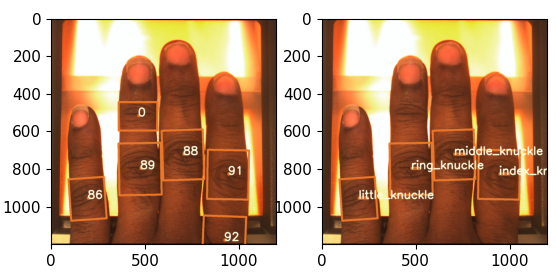
\includegraphics[width=3.25in]{Figure/11-11-2022/select_1.png}
        \label{}
    }
    \subfloat[]{
        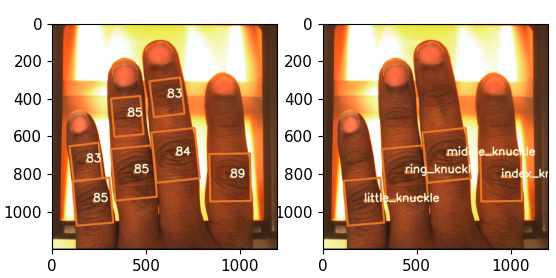
\includegraphics[width=3.25in]{Figure/11-11-2022/select_2.png}
        \label{}
    }

    \subfloat[]{
        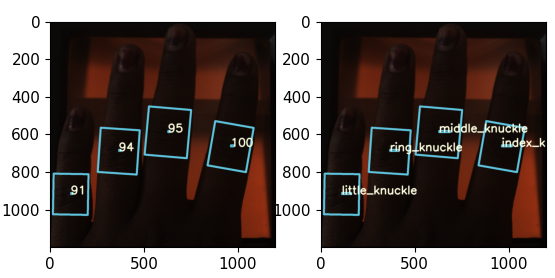
\includegraphics[width=3.25in]{Figure/11-11-2022/select_5.png}
        \label{}
    }
    \subfloat[]{
        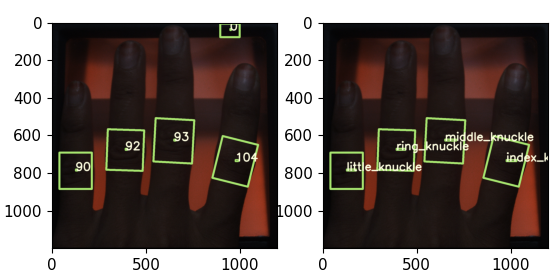
\includegraphics[width=3.25in]{Figure/11-11-2022/select_6.png}
        \label{}
    }

    \caption{After detected by YOLOv5, I follow the same method on the report to select the little, ring, middle, and index finger knuckle based on the geometry of finger.}
    \label{select-algorithm}
\end{figure}




\subsection{Compare the performance between RFN-MSE and RFN-RSIL}


\begin{figure}[h]
    \centering
    \subfloat[]{
        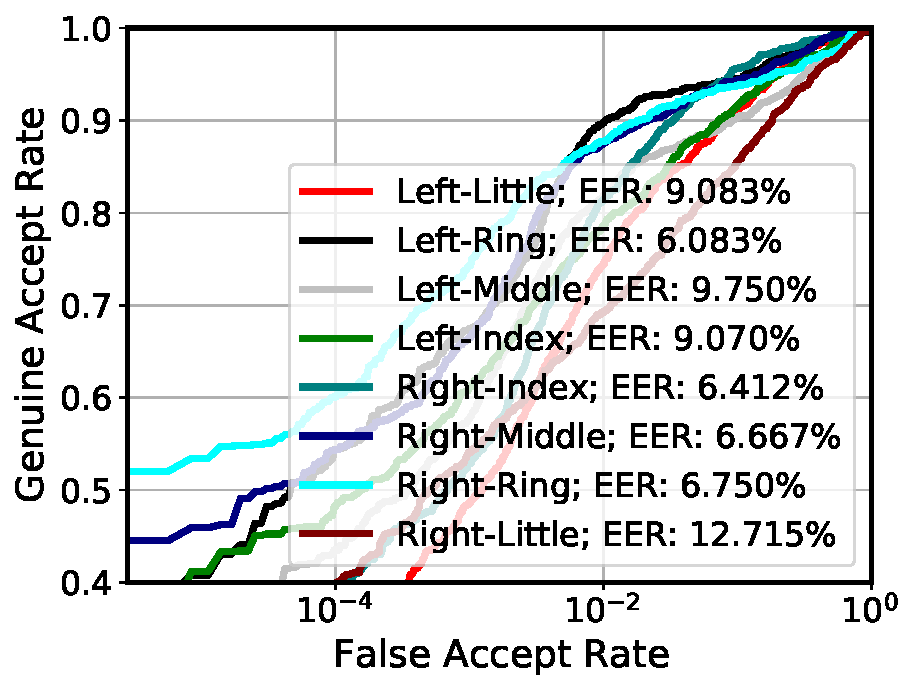
\includegraphics[width=2.8in]{Figure/11-11-2022/rfn-roc.pdf}
        \label{}}
    \subfloat[]{
        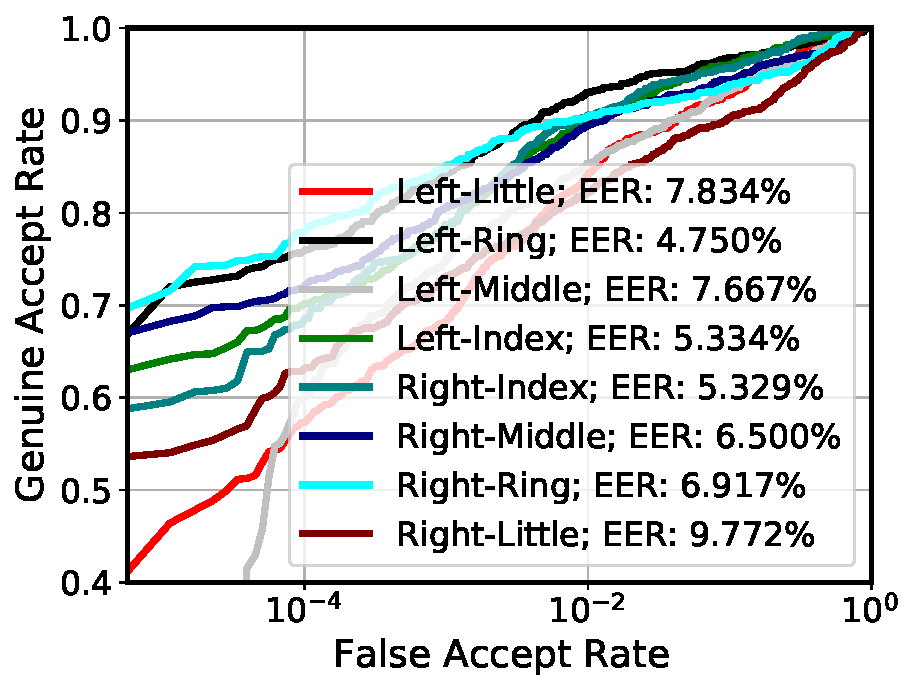
\includegraphics[width=2.8in]{Figure/11-11-2022/rfn-rsil-roc.pdf}
        \label{}}

    \caption{Matching performance of RFN with loss function (a) MSE, (b) RSIL}
    \label{rfn-roc}
\end{figure}

\subsection{Fuse finger knuckle and fingerprint score}
\subsubsection{Dynamic Fusion Fig. \ref{dynamic}, Holistic Fusion Fig. \ref{holistic}, Nonlinear Fusion Fig. \ref{nonlinear}}
\begin{figure}[ht!]
    \centering
    \subfloat[]{
        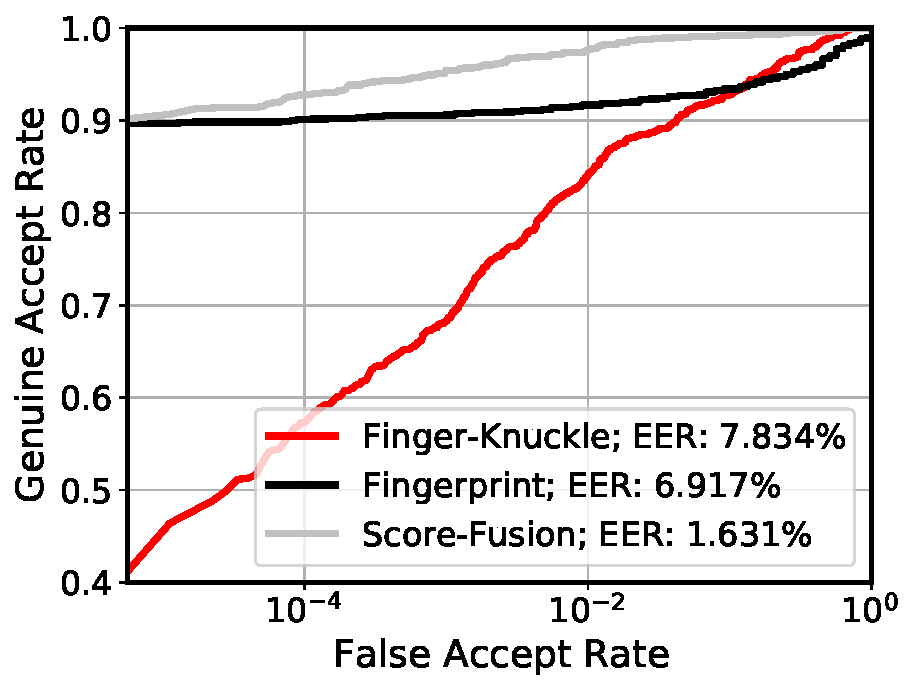
\includegraphics[width=1.9in]{Figure/11-11-2022/dynamic/01.pdf}
        \label{}
    }
    \subfloat[]{
        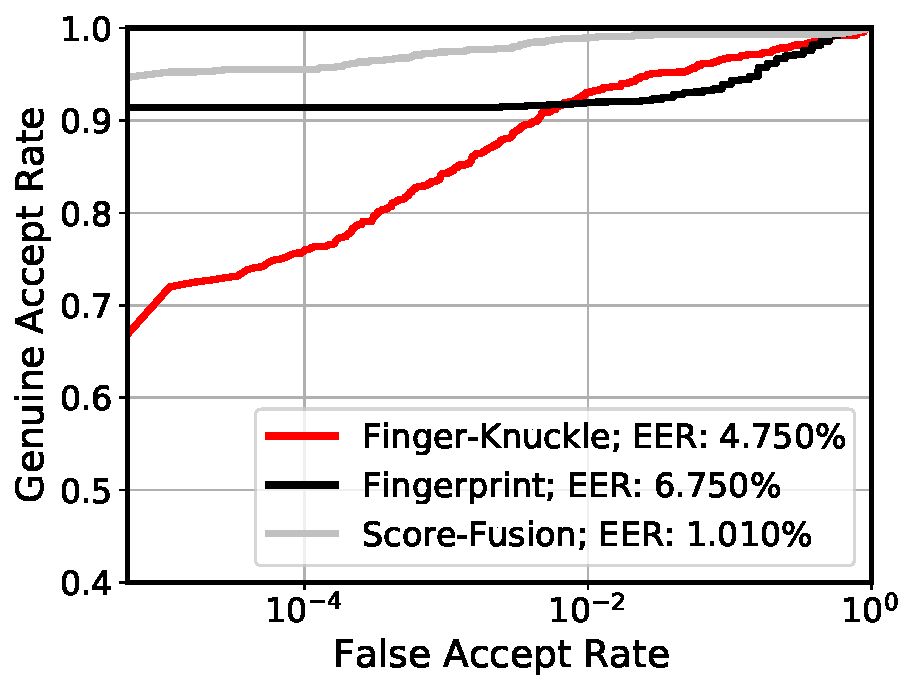
\includegraphics[width=1.9in]{Figure/11-11-2022/dynamic/02.pdf}
        \label{}
    }
    \subfloat[]{
        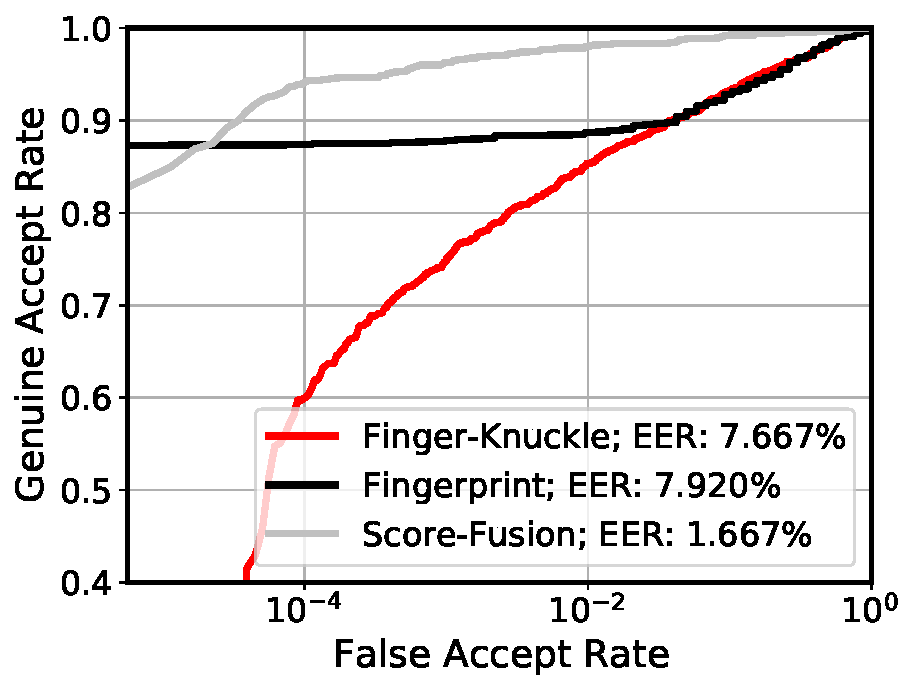
\includegraphics[width=1.9in]{Figure/11-11-2022/dynamic/03.pdf}
        \label{}
    }

    \subfloat[]{
        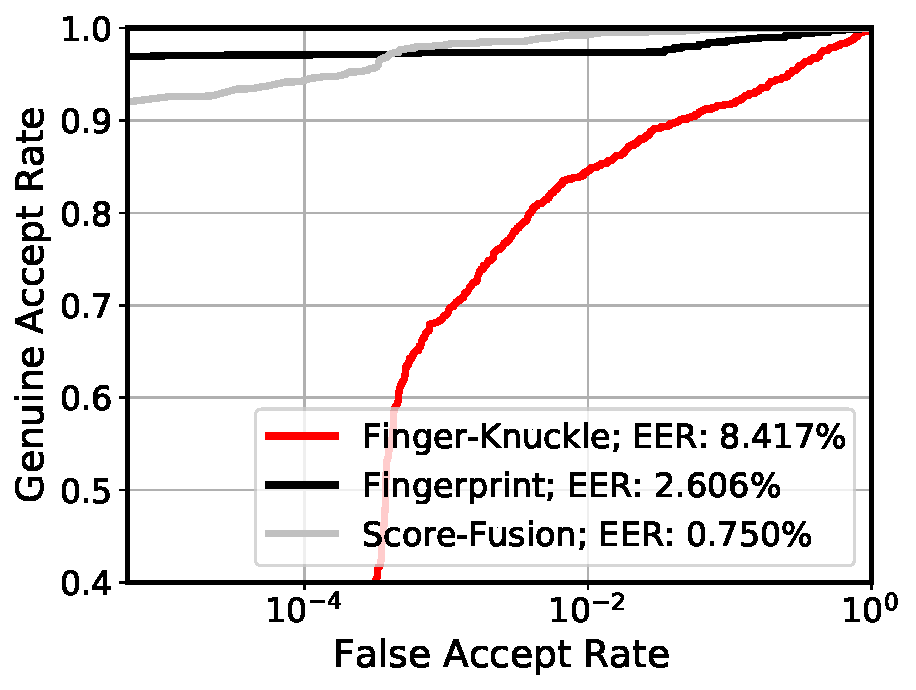
\includegraphics[width=1.9in]{Figure/11-11-2022/dynamic/07.pdf}
        \label{}
    }
    \subfloat[]{
        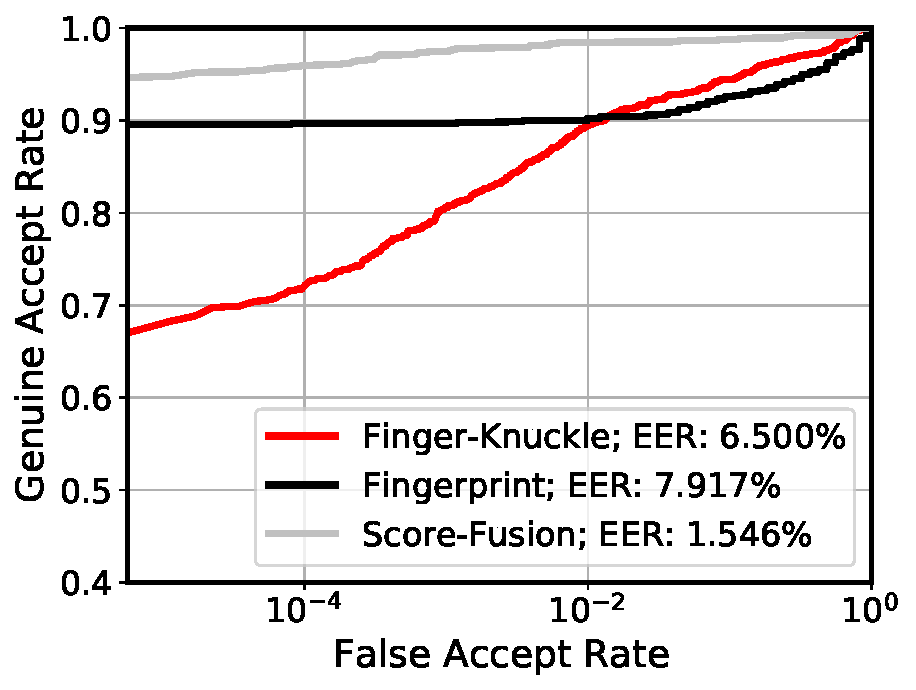
\includegraphics[width=1.9in]{Figure/11-11-2022/dynamic/08.pdf}
        \label{}
    }
    \subfloat[]{
        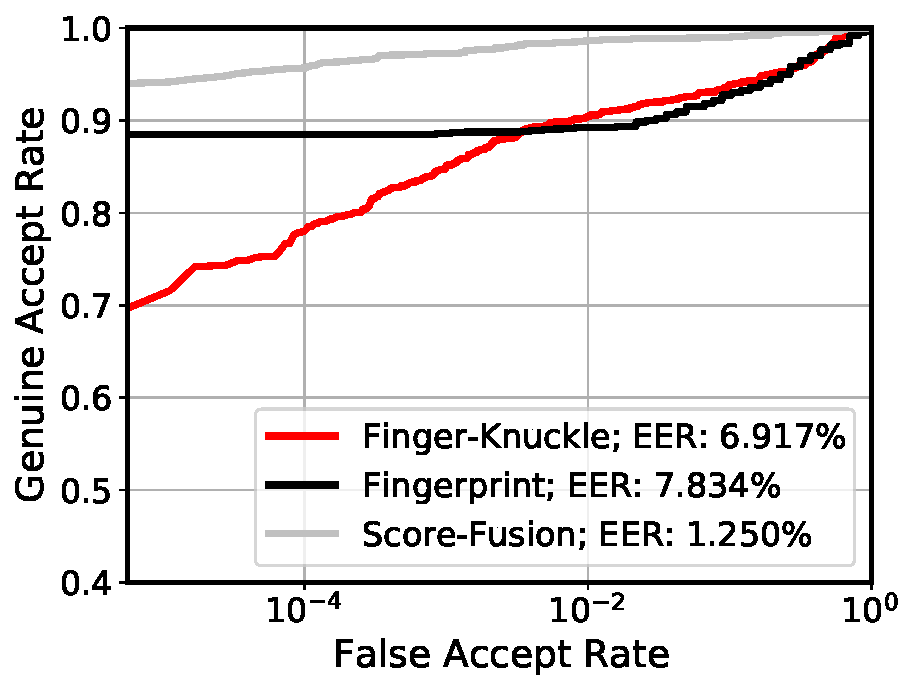
\includegraphics[width=1.9in]{Figure/11-11-2022/dynamic/09.pdf}
        \label{}
    }
    \caption{Using the dynamic score fusion, it is just linear transform between finger knuckle score and fingerprint score. (a) left little finger, (b) left ring finger, (c) left middle finger, (d) right index finger, (e) right middle finger, (f) right ring finger}
    \label{dynamic}
\end{figure}


\begin{figure}[h]
    \centering
    \subfloat[]{
        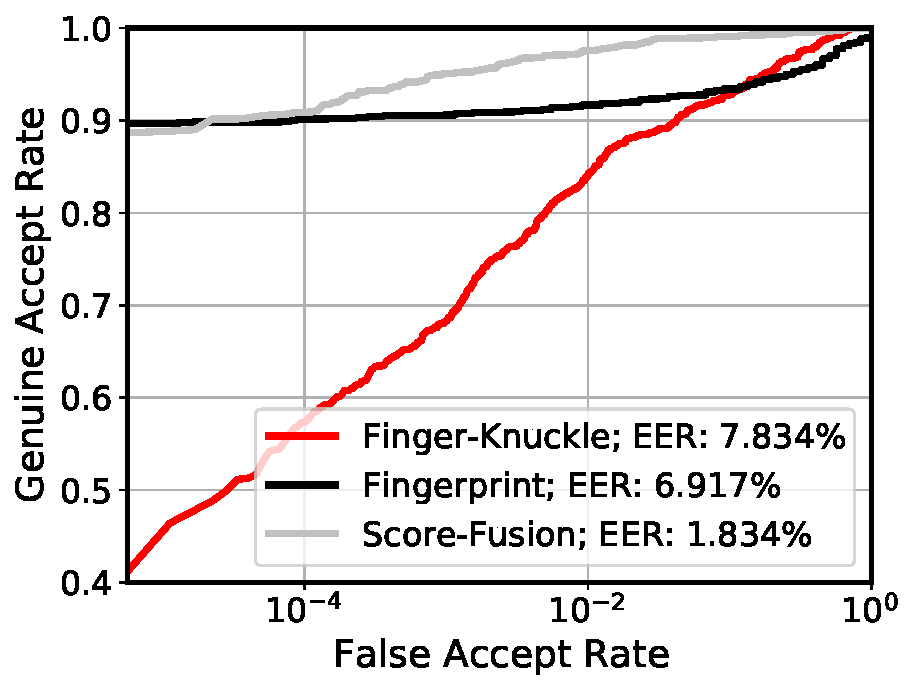
\includegraphics[width=1.8in]{Figure/11-11-2022/holistic/01.pdf}
        \label{}
    }
    \subfloat[]{
        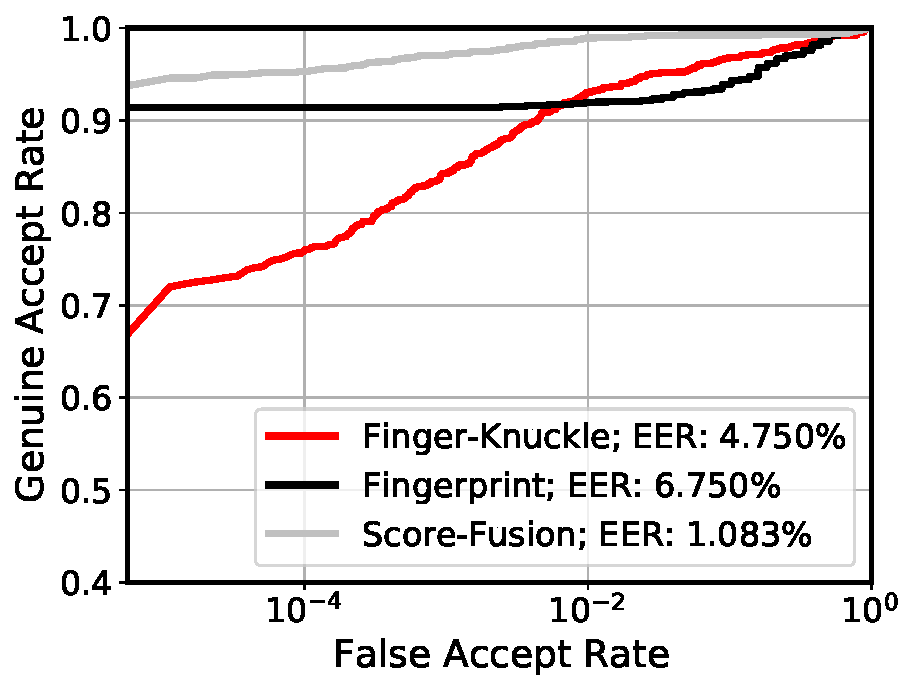
\includegraphics[width=1.8in]{Figure/11-11-2022/holistic/02.pdf}
        \label{}
    }
    \subfloat[]{
        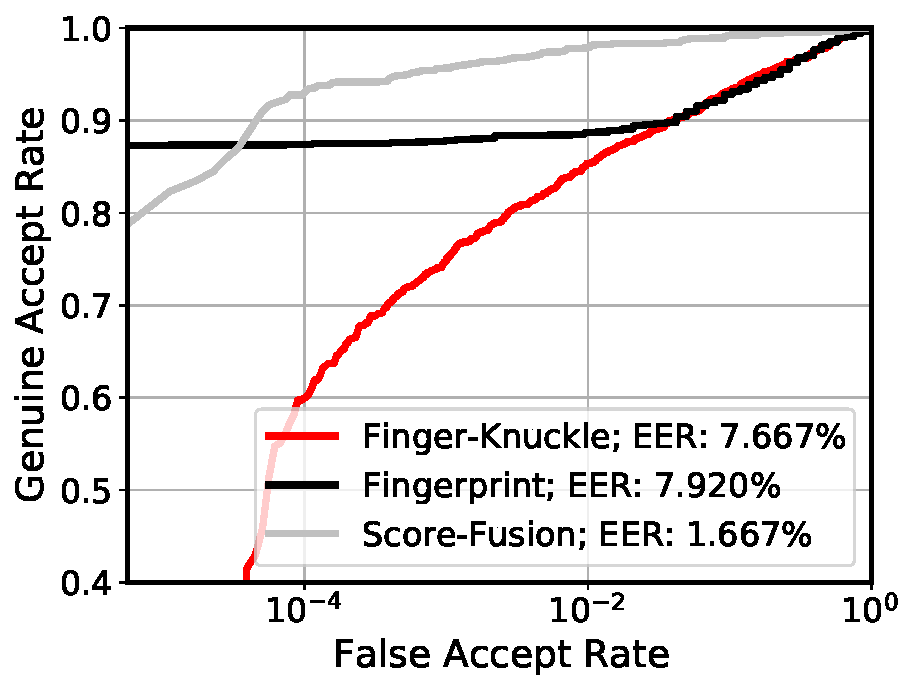
\includegraphics[width=1.8in]{Figure/11-11-2022/holistic/03.pdf}
        \label{}
    }

    \subfloat[]{
        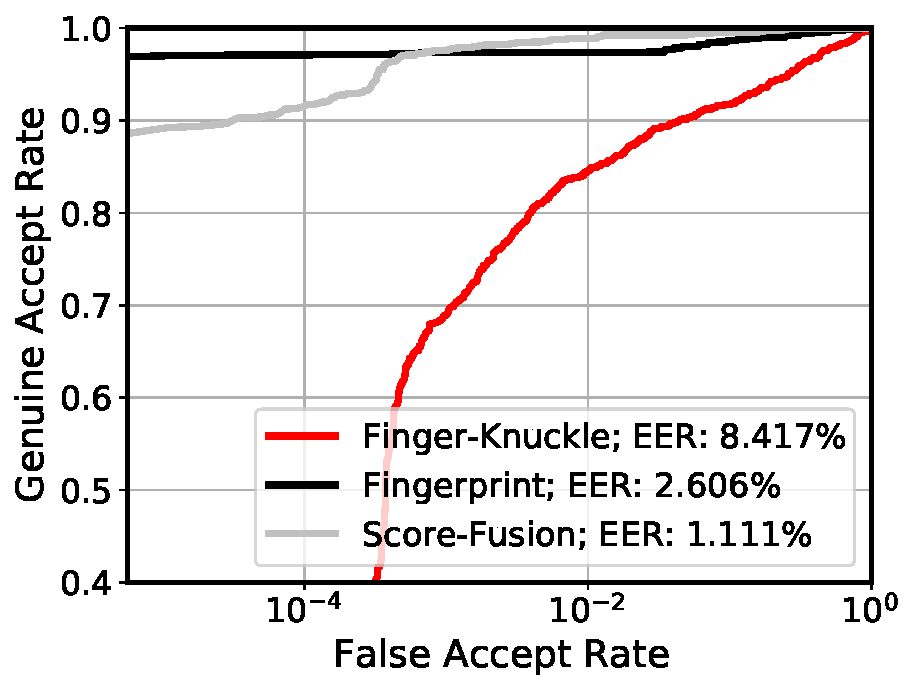
\includegraphics[width=1.8in]{Figure/11-11-2022/holistic/07.pdf}
        \label{}
    }
    \subfloat[]{
        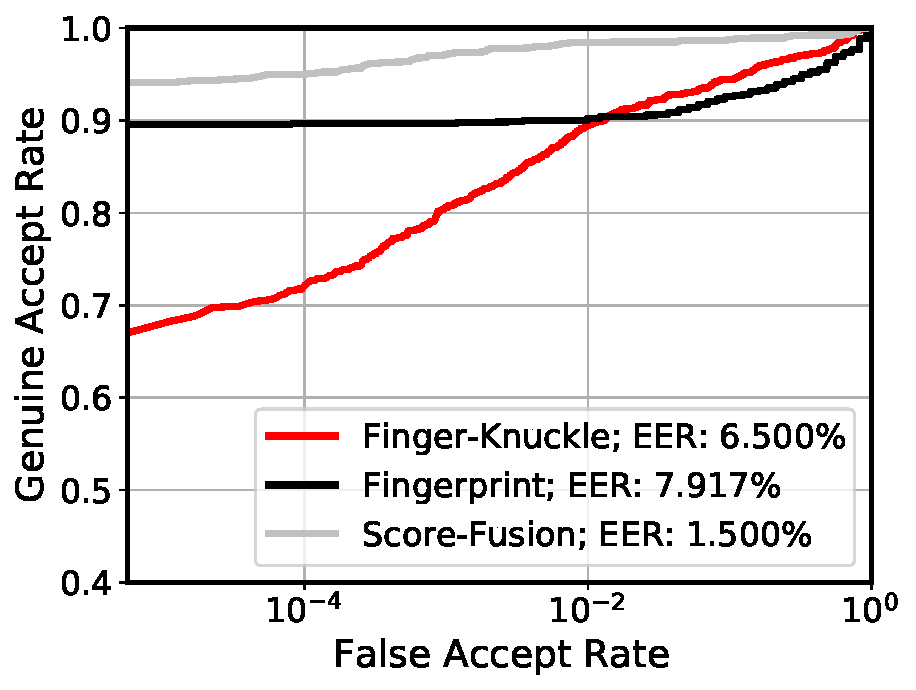
\includegraphics[width=1.8in]{Figure/11-11-2022/holistic/08.pdf}
        \label{}
    }
    \subfloat[]{
        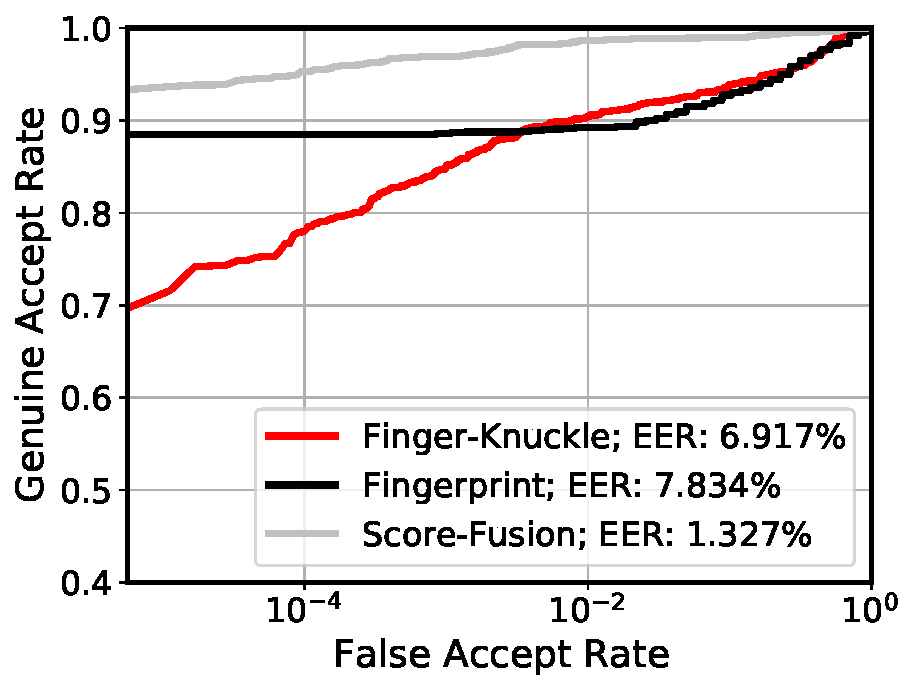
\includegraphics[width=1.8in]{Figure/11-11-2022/holistic/09.pdf}
        \label{}
    }
    \caption{Using the holistic fusion. (a) left little finger, (b) left ring finger, (c) left middle finger, (d) right index finger, (e) right middle finger, (f) right ring finger}
    \label{holistic}
\end{figure}

\begin{figure}[h]
    \centering
    \subfloat[]{
        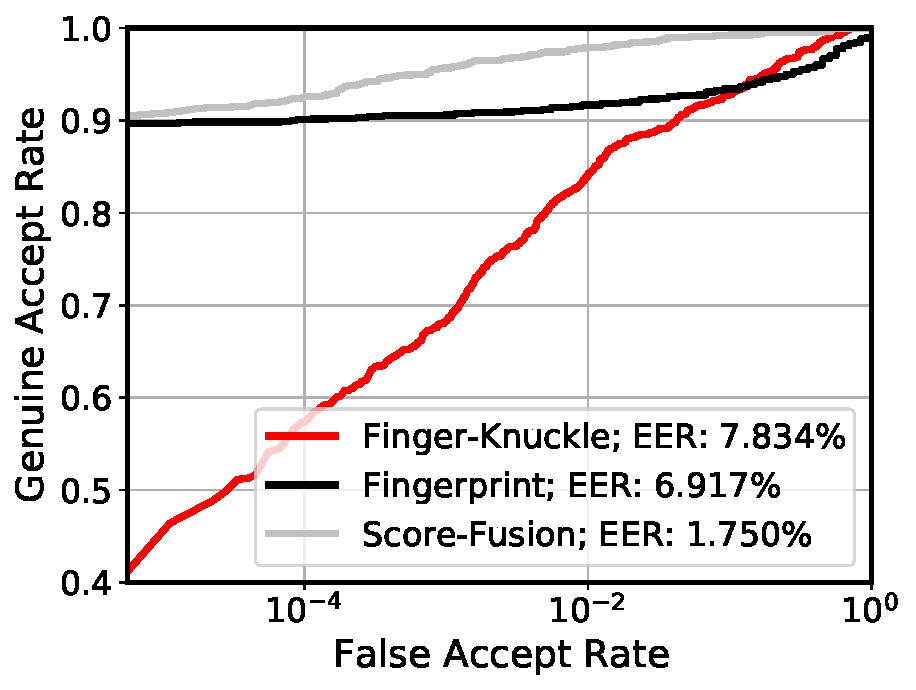
\includegraphics[width=1.8in]{Figure/11-11-2022/nonlinear/01.pdf}
        \label{}
    }
    \subfloat[]{
        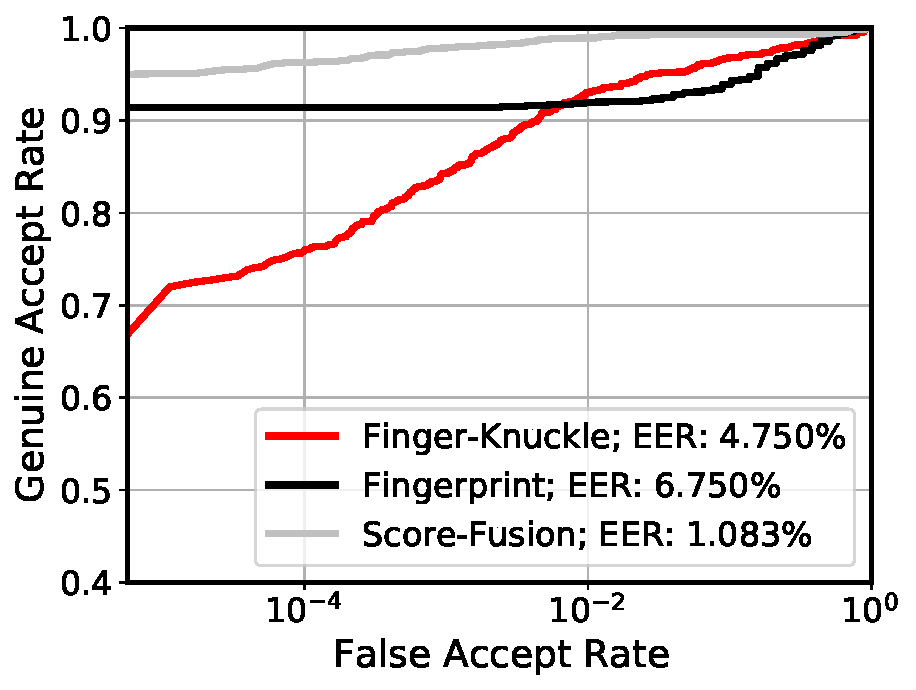
\includegraphics[width=1.8in]{Figure/11-11-2022/nonlinear/02.pdf}
        \label{}
    }
    \subfloat[]{
        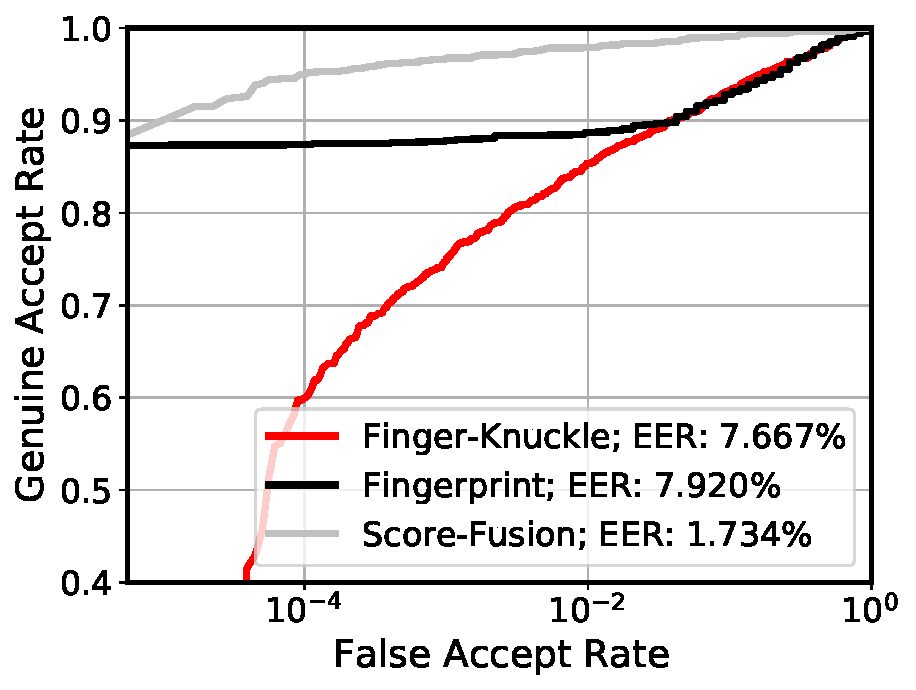
\includegraphics[width=1.8in]{Figure/11-11-2022/nonlinear/03.pdf}
        \label{}
    }

    \subfloat[]{
        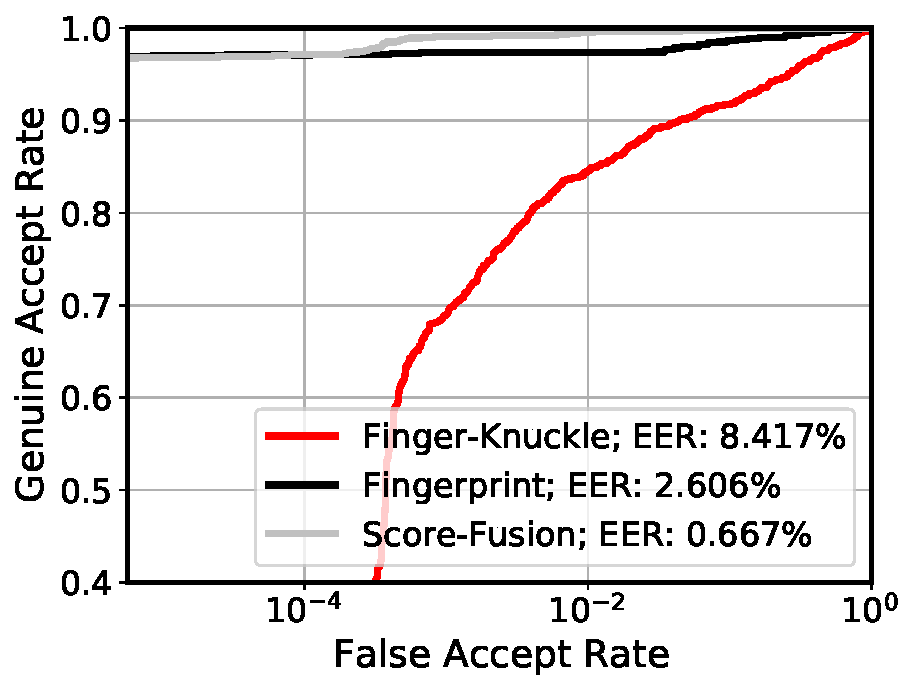
\includegraphics[width=1.8in]{Figure/11-11-2022/nonlinear/07.pdf}
        \label{}
    }
    \subfloat[]{
        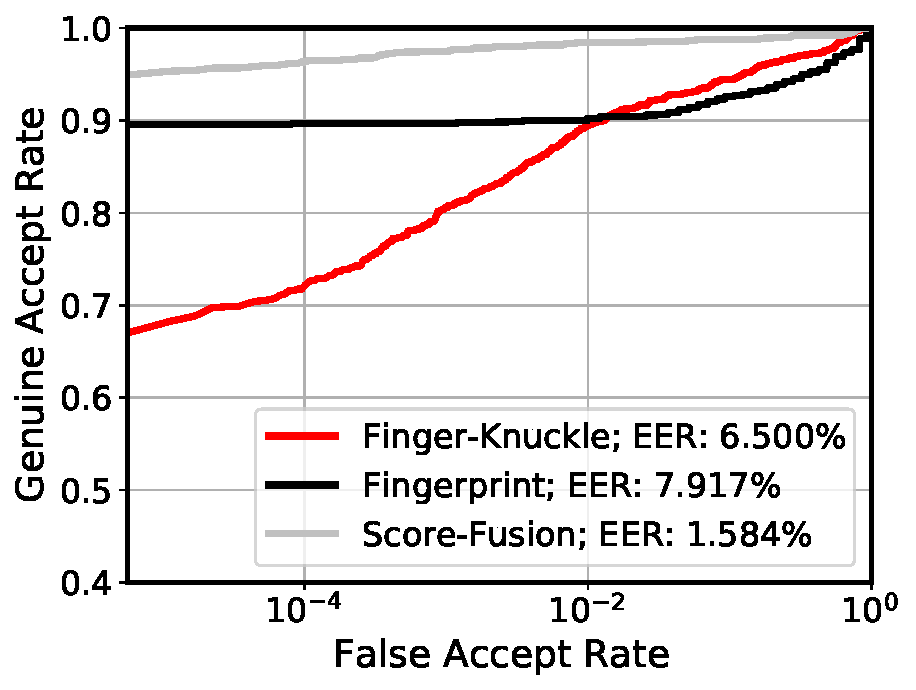
\includegraphics[width=1.8in]{Figure/11-11-2022/nonlinear/08.pdf}
        \label{}
    }
    \subfloat[]{
        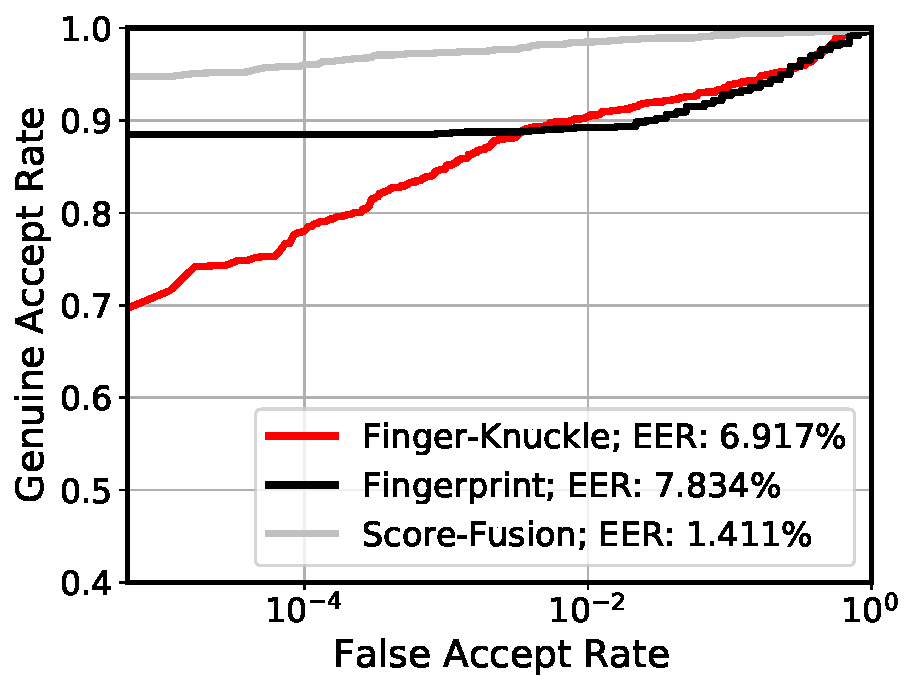
\includegraphics[width=1.8in]{Figure/11-11-2022/nonlinear/09.pdf}
        \label{}
    }
    \caption{Using the holistic fusion. (a) left little finger, (b) left ring finger, (c) left middle finger, (d) right index finger, (e) right middle finger, (f) right ring finger}
    \label{nonlinear}
\end{figure}